\chapter{Nombres relatifs}

\section{Rappels}

\addexo{Construire une droite graduée (axe des abscisses) et y placer le plus précisément possible les événements suivants\,:
\begin{enumerate}[label=\Alph*)]
	\item le temple de Jérusalem est détruit en 70 après Jésus-Christ;
	\item Jules César naît en 100 avant J.-C.;
	\item Constantin crée Constantinople en 324 après J.-C.;
	\item Alexandre le Grand meurt en 324 avant J.-C.
\end{enumerate}
}{-}

Les nombres relatifs (positifs et négatifs) peuvent être représentés sur une droite graduée,  appelée \textbf{(axe des) abscisse(s)}.

\addexo{Construire une droite graduée et placer les points suivants.
$$ A(+3); B(-3); C(-3,5);  $$
$$ D(+3,5); E(+2,5); F(-2,5). $$
}{-}

\addexo{Construire une droite graduée et placer les points suivants.
$$ M(+200); N(-400); P(-250); $$
$$ Q(+300); R(+50). $$
}{-}

\addexo{Construire une droite graduée et placer les points suivants.
$$ S(+3\,500); T(-4\,000); U(-1\,500); $$
$$ V(+3\,000); W(-2\,500). $$
}{-}

\prop{Le nombre 0 est à la fois positif et négatif.
}

\addexo{Recopier et compléter par \og <\fg{} ou \og >\fg.
\begin{enumerate}
	\item $ -5,5 \ldots -2,5 $
	\item $ +2,5 \ldots -5,5 $
	\item $ -4 \ldots +4,5 $
	\item $ -5,5 \ldots -0,5 $
	\item $ +1,5 \ldots -1,5 $
	\item $ -0,5 \ldots +1,5 $
\end{enumerate}
}{-}

\defn{L'\textbf{ensemble des entiers relatifs} (positifs et négatifs), noté $\mathbb{Z}$, avec
$$ \mathbb{Z} = \{... ; -3; -2; -1; 0; 1; 2; 3; ... \} $$
}

%Ex. 7, 8, 9 p.50 \datei{Bicher/T5/T5_p.050.jpg} \\
%Ex. 10 p.51      \datei{Bicher/T5/T5_p.051.jpg} \\
%Ex. 29, 30, 32, 34, 36 p.52   \datei{Bicher/T5/T5_p.052.jpg} \\
%Ex. 39, 40, 42, 43 p.53   \datei{Bicher/T5/T5_p.053.jpg}

\addexo{Ranger par ordre croissant.
$$ +3,5;\, -6;\, -6,5;\, +4;\, -4,5;\, -4;\, -7. $$
}{-}

\addexo{Ranger par ordre décroissant.
$$ +8,72;\, -4,3;\, +8,6;\, +8,5;\, 0;\, -4,72.  $$
}{-}

\addexo{Si possible, compléter par un entier relatif tel que l'inégalité soit vraie.
\begin{enumerate}
	\item $ 4 < \ldots < 6 $
	\item $ -4< \ldots < -2 $
	\item $-2 < \ldots < 0  $
	\item $ -1 < \ldots < 1  $
	\item $ -1,1 < \ldots < -2,1 $
	\item $ -7,1 < \ldots < -6,9 $
\end{enumerate}
}{-}

\addexo{Trouver, si possible, un nombre\,: 
\begin{enumerate}
	\item négatif plus petit que $(-15)$\,;
	\item négatif plus grand que $(-4)$\,;
	\item plus petit que $(-4)$ et plus grand que $(-7)$\,;
	\item plus petit que $(-3)$ et plus grand que $(+1)$\,;
	\item plus petit que 0 et plus grand que $(-4)$\,;
	\item plus petit que $(-7)$ et plus grand que $(-5)$\,;
\end{enumerate}	
}{-}


On peut définir un deuxième axe coupant l'axe des abscisses en $0$.
Cet axe est appelé \textbf{axe des ordonnées}.

\textbf{Exemple\,:}
\begin{center}
\definecolor{xdxdff}{rgb}{0.49,0.49,1}
\definecolor{ffttqq}{rgb}{1,0.2,0}
\definecolor{qqqqff}{rgb}{0,0,1}
\definecolor{qqcctt}{rgb}{0,0.8,0.2}
\definecolor{cqcqcq}{rgb}{0.75,0.75,0.75}
\begin{tikzpicture}[scale=.8, line cap=round,line join=round,>=triangle 45,x=1.0cm,y=1.0cm]
	\draw [color=cqcqcq,dash pattern=on 2pt off 2pt, xstep=1.0cm,ystep=1.0cm] (-3,-3) grid (3,5);
	\draw[->,color=black] (-3,0) -- (3,0);
	\foreach \x in {-3,-2,-1,1,2}
	\draw[shift={(\x,0)},color=black] (0pt,2pt) -- (0pt,-2pt) node[below] {\footnotesize $\x$};
	\draw[->,color=black] (0,-3) -- (0,5);
	\foreach \y in {-3,-2,-1,1,2,3,4}
	\draw[shift={(0,\y)},color=black] (2pt,0pt) -- (-2pt,0pt) node[left] {\footnotesize $\y$};
	\draw[color=black] (-10pt,-10pt) node[right] {\footnotesize $O(0,0)$};
	\clip(-3,-3) rectangle (3,5);
	\draw [->,color=qqcctt] (0,0) -- (2,0);
	\draw [->,color=ffttqq] (2,0) -- (2,3);
	\draw [->,color=qqcctt] (0,0) -- (-2,0);
	\draw [->,color=ffttqq] (-2,0) -- (-2,4);
	\draw [->,color=qqcctt] (0,0) -- (-1,0);
	\draw [->,color=ffttqq] (-1,0) -- (-1,-2);
	\fill [color=qqqqff] (2,3) circle (1.5pt);
	\draw[color=qqqqff] (2.12,3.23) node {$A(2;3)$};
	\fill [color=xdxdff] (-2,0) circle (1.5pt);
	\fill [color=qqqqff] (-2,4) circle (1.5pt);
	\draw[color=qqqqff] (-1.87,4.24) node {$B(-2;4)$};
	\fill [color=qqqqff] (-1,-2) circle (1.5pt);
	\draw[color=qqqqff] (-1.3,-2.3) node {$C(-1;-2)$};
\end{tikzpicture}
\end{center}
\id{vocabulaire\,: abscisse, ordonnée, origine, coordonnées}

Un repère est subdivisé en quatre sous-aires, appelés \textbf{quadrants}\,:
\begin{center}
\definecolor{xdxdff}{rgb}{0.49,0.49,1}
\definecolor{ffttqq}{rgb}{1,0.2,0}
\definecolor{qqqqff}{rgb}{0,0,1}
\definecolor{qqcctt}{rgb}{0,0.8,0.2}
\definecolor{cqcqcq}{rgb}{0.75,0.75,0.75}
\begin{tikzpicture}[scale=0.525, line cap=round,line join=round,>=triangle 45,x=1.0cm,y=1.0cm]
%	\draw [color=cqcqcq,dash pattern=on 2pt off 2pt, xstep=1.0cm,ystep=1.0cm] (-2.9,-2.9) grid (2.9,2.9);
	\draw[->,color=black] (-3,0) -- (3,0);
%	\foreach \x in {-3,-2,-1,1,2}
%	\draw[shift={(\x,0)},color=black] (0pt,2pt) -- (0pt,-2pt) node[below] {\footnotesize $\x$};
	\draw[->,color=black] (0,-3) -- (0,3);
%	\foreach \y in {-3,-2,-1,1,2}
%	\draw[shift={(0,\y)},color=black] (2pt,0pt) -- (-2pt,0pt) node[left] {\footnotesize $\y$};
	\draw[color=black] (-0pt,-10pt) node[right] {\footnotesize $0$};
	\clip(-3,-3) rectangle (3,3);
	\draw[color=qqqqff] ( 1.5, 1.5) node {1er q.};
	\draw[color=qqqqff] (-1.5, 1.5) node {2e q.};
	\draw[color=qqqqff] (-1.5,-1.5) node {3e q.};
	\draw[color=qqqqff] ( 1.5,-1.5) node {4e q.};
\end{tikzpicture}
\end{center}


\rem{Avec 2 axes, on peut repérer des points dans un plan (2d), \\
Avec 3 axes, on peut repérer des points dans l'espace (3d) [$\rightarrow$ section TG].
}

\defn{Dans un repère du plan, la position d'un point est représentée par deux nombres relatifs\,:
\begin{itemize}
  \item Le premier est lu sur l'axe des abscisses. Ce nombre est appelé \textbf{abscisse}.
  \item Le deuxième est lu sur l'axe des ordonnées. Ce nombre est appelé \textbf{ordonnée}.
\end{itemize}
Les deux nombres sont les \textbf{coordonnées} du point.
}

%\arrow Ex. 18, 19, 20, 21, 22 p.51 (placer les points) \datei{Bicher/T5/T5_p.051.jpg} \\
%\arrow Ex. 50 p.54 (énigme) \datei{Bicher/T5/T5_p.054.jpg}

\addexo{Dans quel quadrant sont situés les points suivants\,?
$$ A(2,6;-3);\, B(-2; 3,4); $$
$$ C(-2,6;-3,5);\, D(6,4;2,3). $$
}{-}

\addexo{Dans quel quadrant sont situés les points suivants\,?
$$ P(+3\,000;-500);\, Q(-500; -3\,000); $$
$$ R(-500; +3\,000);\, S(+100; +200). $$
}{-}

\addexo{Soit la figure ci-dessous.
\begin{enumerate}
	\item Quelle est l'abscisse de $E$\,?
	\item Quelle est l'ordonnée du point $E$\,?
	\item Quelles sont les coordonnes des autres points\,?
\end{enumerate}
\begin{center}
	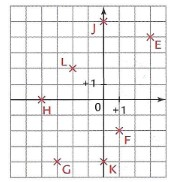
\includegraphics[width=4.5cm]{pictures/pts_dans_le_plan}
\end{center}
}{-}

\addexo{Soit la figure ci-dessous.
\begin{enumerate}
	\item Quel point a pour abscisse $+2$\,?
	\item Quel point a pour ordonnée $-2$\,?
	\item Quelles sont les coordonnes des points $G,A,B$ et $F$\,?
	\item Nommer deux points qui ont la même abscisse.
	\item Nommer deux points qui ont la même ordonnée.
\end{enumerate}
\begin{center}
	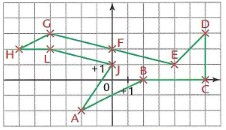
\includegraphics[width=6cm]{pictures/pts_dans_le_plan2}
\end{center}
}{-}

\addexo{Placer les points suivants dans un repère.
$$ A(+5; +4);\, B(+5;+8); C(-3;+4); D(-3;+8). $$
Quelle est la nature du quadrilatère $ABDC$\,?
Et de $ABCD$\,?
}{-}

\addexo{Sur une droite graduée, quelle est la distance des nombres $2; 5; -4; -57$ et l'origine $0$\,?
}{-}

\addexo{Indiquer la valeur absolue des nombres suivants\,:
2; 5; $-4$; $-57$.
}{On note\,: $|2|=2$, $|5|=5$, $|-4|=4$, $|-57|=57$.
}

\defn{La \textbf{valeur absolue} d'un nombre est sa valeur numérique sans tenir compte de son signe.
}


\section{Somme de nombres relatifs}

\addexo{Dans un jeu vidéo, on joue toujours deux parties.
On peut gagner ou perdre des points, marqués par des nombres positifs ou négatifs.
Le tableau ci-dessous regroupe les résultats de quelques jeux de Pierre.
\begin{center}
\begin{tabular}{c|c|c}
	Jeu & 1$^{re}$ partie & 2$^e$ partie \\
	\hline
	a) & +3 & +7 \\
	b) & +9 & +3  \\
	c) & $-4$ & $-2$ \\
	d) & $-5$ & $-6$
\end{tabular}
\end{center}
Effectuer le bilan pour chaque jour en notant chaque fois le calcul associé.
}{-}

\ret{Pour ajouter deux nombres de même signe,
\begin{enumerate}
	\item on garde le signe et
	\item on ajoute leurs valeurs absolues.
\end{enumerate}	
}
\rem{Lorsqu'on a deux signes consécutifs, on doit mettre des parenthèses.
}

\addexo{Ci-dessous sont les résultats de Julie pour le même jeu vidéo.
\begin{center}
\begin{tabular}{c|c|c}
	Jeu & 1$^{re}$ partie & 2$^e$ partie \\
	\hline
	a) & +8 & $-5$ \\
	b) & $-3$ & +7  \\
	c) & $-12$ & $+11$ \\
	d) & $+3$ & $-7$
\end{tabular}
\end{center}
Effectuer le bilan pour chaque jour en notant chaque fois le calcul associé.
}{-}

\ret{Pour ajouter deux nombres de signes contraire,
\begin{enumerate}
	\item on note le signe du nombre relatif ayant la plus grande valeur absolue et
	\item on retranche la plus petite valeur absolue de la plus grande.
\end{enumerate}
}

\addexo{Effectuer les calculs suivants.
\begin{enumerate}
	\item $ (-13)+(+10)= $
	\item $ (-7)+(-4)= $
	\item $ (+9)+(-12)= $
	\item $ (-12)+(+13)= $
	\item $ (+18)+(-24)= $
	\item $ (-46)+(+46)= $
\end{enumerate}
}{-}
\defn{Deux nombres relatifs dont la somme est 0 sont appelés \emph{nombres opposés}.
}

\addexo{Effectuer les calculs suivants.
\begin{enumerate}
	\item $ (-8)+(+12)= $
	\item $ (+9)+(-13)= $
	\item $ (+5)+(-4)= $
	\item $ (-16)+(-18)= $
	\item $ (-17)+(+6)= $
	\item $ (-12)+(+3)= $
\end{enumerate}
}{-}

\addexo{Effectuer les calculs suivants.
\begin{enumerate}
	\item $ (+15)+(-17)= $
	\item $ (-98)+(-3)= $
	\item $ (-75)+(+19)= $
	\item $ (+81)+(-8)= $
	\item $ (+17)+(-21)= $
	\item $ (-23)+(-24)= $
\end{enumerate}
}{-}

\addexo{Effectuer les calculs suivants.
\begin{enumerate}
	\item $ (+65)+(-17)= $
	\item $ (-28)+(-13)= $
	\item $ (+9)+(-36)= $
	\item $ (+18)+(-19)= $
	\item $ (+75)+(-26)= $
	\item $ (-48)+(-42)= $
\end{enumerate}
}{-}

\addexo{Effectuer les calculs suivants.
\begin{enumerate}
	\item $ (-2,45)+(+3,84)= $
	\item $ (+7,8)+(-5,2)= $
	\item $ (+8,1)+(-9,3)= $
	\item $ (-24,8)+(-2,7)= $
	\item $ (-54,2)+(+45,9)= $
	\item $ (+97,5)+(-54,7)= $
\end{enumerate}
}{-}

\addexo{Effectuer les calculs suivants.
\begin{enumerate}
	\item $ (+1,01)+(-1,1)= $
	\item $ (-15,8)+(+23,7)= $
	\item $ (-1)+(+0,1)= $
	\item $ (-58,8)+(-12,2)= $
	\item $ (-99,9)+(+0,01)= $
	\item $ (+12,05)+(-13,07)= $
\end{enumerate}
}{-}

\addexo{Compléter.
\begin{enumerate}
	\item $ (+9,2)+\ldots = -5 $
	\item $ \ldots+(-0,5) = -0,4 $
	\item $ \ldots +(+1,9) = 0 $
	\item $ (-2,01)+\ldots = 0 $
	\item $ (-0)+\ldots = -52,7 $
	\item $ \ldots +(+7,15) = +6,12 $
\end{enumerate}
}{-}

\addexo{Effectuer les calculs suivants.
\begin{enumerate}
	\item $ (-15)+(-9)+(+8)+(-12)+(-8)= $
	\item $ (+91)+(-57)+(+15)+(-26)= $
	\item $ (-13)+(+24)+(+45)+(-49)+(-24)= $
	\item $ (+47)+(-45)+(-87)+(+62)+(+78)= $
	\item $ (-29)+(-74)+(+42)+(-101)+|-17|= $
	\item $ (-76)+(-12)+(+98)+(-45)+|+21|+(+112)= $
\end{enumerate}
}{-}

\ret{Pour effectuer une somme, on peut déplacer les termes dans l'ordre que l'on veut.
C'est la commutativité de l'addition.
}

%\arrow Ex. 22*, 23, 24*, 30, 31*, 32* p.80 ($\Delta$5e)

\addexo{Effectuer les calculs suivants.
\begin{enumerate}
	\item $ (-18)+(-12)+(-11)+(+18)+(+13)= $
	\item $ (-52)+(+48)+(-60)+(+4)= $
	\item $ (+78)+(-60)+(+1)+(-18)= $
	\item $ (+121)+(-88)+(-71)+(+25)+(+8)= $
	\item $ (-19)+(+80)+(-51)+(-55)= $
	\item $ (-324)+(+547)+|-124|+(-327)= $
\end{enumerate}
}{-}

\addexo{Effectuer les calculs suivants.
\begin{enumerate}
	\item $ (+2,8)+(-7,9)+(-2,3)+(+19,2)= $
	\item $ (+1,1)+(-2,2)+(+3,3)+(-4,4)= $
	\item $ (-12,07)+(+19,8)+(-25,4)+(-9,7)+(-1,87) =$
	\item $ (-1,08)+(-2,71)+(+3,87)= $
	\item $ (+15,09)+(+14,3)+(+27,8)+(-0,1)+(-0,09)= $
	\item $ (-27,8)+(-17,05)+(+24,8)+(+16)+(+0,06)+(-0,01)= $
\end{enumerate}
}{-}

\addexo{Calculer mentalement.
\begin{enumerate}
	\item $ (-183)+(+7)+(+12)+(-4)+(+183)= $
	\item $ (-54)+(+87)+(+3)+(+54)+(-87)= $
	\item $ (+68)+(-38)+(-2)+(-68)+(+38)= $
	\item $ (-19)+(-12)+(+19)+(+53)+(+12)= $
	\item $ (+21)+(+47)+(-15)+(-47)+(+9)= $
	\item $ (-64)+(+12)+(-23)+(-8)+(+23)= $
\end{enumerate}
}{-}


%\arrow Ex. 7, 8, 9, 10*, 11*,  p.79 ($\Delta$5e) \datei{Bicher/T5/T5_p.079.jpg} \\
%\arrow Ex. 26 p.80 (Déf. nombres opposés) \datei{Bicher/T5/T5_p.080.jpg}

\addexo{Compléter tel que l'égalité soit vraie.
\begin{enumerate}
	\item $(-4)+(\ldots)=0$
	\item $(\ldots)+(+8)=0$
	\item $(\ldots)+(-7)=0$
	\item $(+5)+(\ldots)=0$
\end{enumerate}
}{-}

\defn{Deux nombres relatifs sont \textbf{opposés} si leur somme est égale à zéro.
}
Exemples\,:
$3$ et $-3$ sont opposés, ainsi que $1,5$ et $-1,5$. De même\,: $-\frac{1}{3}$ est l'opposé de $\frac{1}{3}$.

%\arrow Ex. 27, 28, (29) p.80 ($\Delta$5e)

\addexo{Trouver la valeur de la lettre dans chaque cas.
\begin{enumerate}
	\item $m+(+8)=0$
	\item $(-4)+p=0$
	\item $r+(-6)=0$
	\item $(+7)+t=0$
\end{enumerate}
}{-}




\section{Différence de nombres relatifs}
\addexo{Dans un jeu, Tim a obtenu des cartes avec les points suivants\,:
$$ +7; \quad -2; \quad +5; \quad -6.  $$
\begin{enumerate}
	\item Déterminer la somme de ses points.
\end{enumerate}
Un autre joueur tire une des cartes de Tim.
\begin{enumerate}[start=2]
	\item Déterminer à l'aide du résultat précédent la nouvelle somme lorsque l'autre joueur a tiré la carte avec $+7$.
	\item Même question si l'autre joueur a tiré la carte avec $-6$.
	\item Même question si l'autre joueur a tiré la carte avec $-2$.
	\item Est-il possible de noter les calculs ci-dessus sous forme d'une addition\,?
\end{enumerate}
}{-}

\noindent
Au lieu de retirer la carte avec $-6$, on peut ajouter +6. \\
Au lieu de retirer $+7$, on peut ajouter $-7$ (nombre opposé).

\noindent
\textbf{Conclusion\,:} Retirer un nombre relatif revient à ajouter l'opposé de ce nombre\,:
$$ -(+a) = +(-a) $$
$$ -(-a) = +(+a) $$


\addexo{Calculer.
\begin{enumerate}
	\item $ (+7)-(-5)-(+4)+(-2)= $
	\item $ (-1)+(-1)-(-2)-(+2)= $
	\item $ (-12)-(-59)+(-45)-(-18)= $
	\item $ (-52)+|-21|-(-17)-(-52)= $
	\item $ (+24)+(-56)-(-47)+(-42)-(+32)-(-99)= $
	\item $ (-427)+(-781)-(-547)-(+155)= $
\end{enumerate}
}{-}

\ret{Pour tout nombre $a$\,:
$$\begin{array}{rcl}
	+(+a) &=& +a  \\
	+(-a) &=& -a  \\
	-(+a) &=& -a  \\
	-(-a) &=& +a 
\end{array}$$
}

%\arrow Ex. 34, 35*, 36*, 37, 38*, 39*,  p.81 \datei{Bicher/T5/T5_p.081.jpg}\\
%\arrow Ex. 43, 44*, 45*, 47 p.81 \\
%\arrow Ex. 48 - 53* p.82 \datei{Bicher/T5/T5_p.082.jpg}

\addexo{Calculer.
\begin{enumerate}
	\item $ (-9)-(-4)= $
	\item $ (-8)-(+3)= $
	\item $ (+7)-(+2)= $
	\item $ (+ 16)-(-3)= $
	\item $ (-5)-(-9)= $
	\item $ (+8)-(+15)= $
\end{enumerate}
}{-}

\addexo{Calculer.
\begin{enumerate}
	\item $ (+4)-(-9)= $
	\item $ (+6)-(-3)= $
	\item $ (-6)-(+8)= $
	\item $ (-9)-(-4)= $
	\item $ (+7)-(+3)= $
	\item $ (+5)-(+9)= $
\end{enumerate}
}{-}

\addexo{Calculer.
\begin{enumerate}
	\item $ (+14)-(-17)= $
	\item $ (+ 26)- (- 18)= $
	\item $ (- 46)-(+38)= $
	\item $ (+17)- (+ 23)= $
	\item $ (-39)-(-14)= $
	\item $ (+35)-(+49)= $
\end{enumerate}
}{-}

\addexo{Trouver la valeur de la lettre dans chaque cas.
\begin{enumerate}
	\item $e-(- 8) = 0$
	\item $f-(+5) = 0$
	\item $(-9)-g = 0$
	\item $h-(+7) = 0$
\end{enumerate}
}{-}

\addexo{Calculer.
\begin{enumerate}
	\item $(- 4,8) + (+ 3,5)=$
	\item $ -2,9)-(-3,2)=$
	\item $(+ 8,2) - (+ 5,6)=$
	\item $(+ 5,8) + (- 2,4)=$
\end{enumerate}
}{-}

\addexo{Calculer.
\begin{enumerate}
	\item $(+ 2,5) + (- 4,5)=$
	\item $(-5,5)-(-3,5)=$
	\item $(+7,5)-(+4,5)=$
	\item $(+6,5)-(+9,5=$
	\item $(- 8,5) + (+ 9,5)=$
	\item $(- 6,5) - (- 8,5)=$
\end{enumerate}
}{-}

\addexo{Calculer.
\begin{enumerate}
	\item $(+ 6,2) - (+ 8,2)=$
	\item $(+ 4,5) - (+ 3,5)=$
	\item $(+8,6)+ (-4,3)=$
	\item $(+9,3) - (- 3,8)=$
	\item $(- 1,8) - (- 1,3)=$
	\item $(- 5,4) + (+ 7,2)=$
\end{enumerate}
}{-}

\addexo{Calculer.
\begin{enumerate}
	\item $(+7)-(-10)=$
	\item $(+6) + (-3)=$
	\item $(-4)-(+12)=$
	\item $(-9)-(-4)=$
	\item $(-17) + (-13)=$
	\item $(+5)-(+9)=$
\end{enumerate}
}{-}


\section{Écriture simplifiée}
Pour effectuer une suite de calculs, on additionne les nombres deux à deux. \\
(Faire un exercice pour montrer le regroupement des nombres deux à deux.) \\

\addexo{Écrire d'abord en écriture simplifiée, puis calculer.
\begin{enumerate}
	\item $ (+1)-(+2)+(-3)-(-4)= $
	\item $ (-1,24)+(-2,59)-(-1,4)= $
	\item $ (+6,75)-(+4,07)+(+4,8)= $
	\item $ (-1,01)+(+2,24)-(+1,98)-(-0,09)= $
	\item $ (+10,2)-(+4,72)-|-1|= $
	\item $ (+9,74)-(-10,21)+(-0,85)-(-0,99)= $
\end{enumerate}
}{-}

\addexo{Calculer.
\begin{enumerate}
	\item $ -12+18-9-12= $
	\item $ 45-13-78+24= $
	\item $ -1,28+5,78-1,22= $
	\item $ -(-0,05+7,54)-2,54-1,7= $
	\item $ -45-(45-8+5)-9 =$
	\item $ 29+(68-73)-32= $
\end{enumerate}
}{-}

\addexo{Calculer mentalement.
\begin{enumerate}
	\item $ 54-108+54= $
	\item $ 30-32+40-50+20= $
	\item $ 72-68+53-72+15= $
	\item $ 98-24-24= $
	\item $ -121+30+22-31= $
	\item $ 35-85+75-15= $
\end{enumerate}
}{-}

\arrow Ex. 101, 102, 105, 106, 107, 109 p.57f (CP)
\\
\arrow Ex. 54 p.82
\\
\arrow Ex. 55', 56*, 57* p.82

Beispiller maan fir di nei convention anzeféiren

\ret[Convention d'écriture]{
Dans une suite d'additions de nombres relatifs, on supprime les \uline{signes d'addition} et les parenthèses autour de chaque nombre. En plus, on peut supprimer le signe d'un nombre positif en début de calcul.
}
\arrow Ex. 58, 59, 60*-62* p.82 \\
%\arrow Ex. 63-65*, 67-70* p.83 \datei{Bicher/T5/T5_p.083.jpg}

Selon disposition du temps\,: problèmes et énigmes.



\section{Multiplication et division de nombres relatifs}
\subsection{Rappels}
\addexo{Joe possède 12 cartes à collectionner.
Il achète 6 paquets, chacun contenant 8 nouvelles cartes. Combien de cartes possède-t-il\,?
}{$12 +\underbrace{6 \cdot 8}_{=48} = 12 + 48 = 60 $  (\og Punkt vor Strich!\fg) \\
Après l'achat, Joe compte 60 cartes.
}

\addexo{Effectuer les calculs suivants.
Indiquer au moins deux facteurs et deux termes.
\begin{multicols}{5}
\noindent
$  11 +10\,:5= \\
  9 \cdot 5 - 8 \cdot 8= \\
  6 \cdot (7 -2)= \\
  4 \cdot 5 -6= \\
  (4 +2\cdot 8) \cdot 5=$
\end{multicols}
}{-}

\ret{Afin d'effectuer une suite de calculs on doit respecter l'ordre suivant\,:
\begin{enumerate}
  \item D'abord, on effectue les calculs entre parenthèses,
  \item ensuite les multiplications et divisions.
  \item Puis les sommes (et les différences).
\end{enumerate}
}

%\arrow Ex. 14 p.17 (T4) \datei{Bicher/T4/T4_p.017.jpg}



\subsection{Règles de calcul}
\stitle{Activité}
$$\begin{array}[t]{ll}
	(+2) \cdot (+3)  =& +6 \\
	(+1) \cdot (+3)  =& +3 \\
	(+0) \cdot (+3)  =&  0 \\
	(-1) \cdot (+3)  =& -3 \\
	(-2) \cdot (+3)  =& -6
\end{array}$$

\ret{Un nombre négatif multiplié par un nombre positif donne un nombre négatif.
}

$$\begin{array}{ll}
	(-2) \cdot (+3)  =& -6 \\
	(-2) \cdot (+2)  =& -4 \\	
	(-2) \cdot (+1)  =& -2 \\
	(-2) \cdot (+0)  =& 0  \\
	(-2) \cdot (-1)  =& +2 \\
	(-2) \cdot (-2)  =& +4	
\end{array}$$

\ret{Pour multiplier/diviser deux nombres relatifs,
on détermine d'\textbf{abord le signe} du produit\,:
$$ \boxed{%
\begin{array}{rrrr}
 (+..) & \cdot & (+..) &=+.. \\
 (+..) & \cdot & (-..) &=-.. \\
 (-..) & \cdot & (+..) &=-.. \\
 (-..) & \cdot & (-..) &=+..
\end{array}
} $$
Ensuite, on multiplie les \textbf{nombres} sans signe.
}

\addexo{Calculer.
\begin{enumerate}
	\item $ (-6)\cdot(+5)= $
	\item $ (-8)\cdot(-7)= $
	\item $ (-12)\cdot(-11)= $
	\item $ (-15)\cdot(+15)= $
	\item $ (+32)\cdot(-25)= $
	\item $ (-50)\cdot(-42)= $
\end{enumerate}
}{-}


\addexo{Calculer.
\begin{enumerate}
	\item $ (-2,5)\cdot(-1,5)= $
	\item $ (+6,7)\cdot(-12)= $
	\item $ (-18)\cdot(+20)= $
	\item $ -9,1\cdot(+11)= $
	\item $ 19\cdot(-3)= $
	\item $ -6\cdot 21= $
\end{enumerate}
}{-}

\rem{Lorsqu'on a deux signes d'opération ($+;-;\cdot;\,:$) consécutifs, alors on doit mettre des parenthèses.
}


À l'aide de la multiplication $(+3)\cdot(-4)=-12$, on obtient deux divisions\,: \\
\begin{center}
	$ (-12)\,:(+3)=-4 $ et $ (-12)\,:(-4)=+3 $.
\end{center}
\ret{Les règles de calcul pour la division correspondent à ceux de la multiplication\,:
\begin{enumerate}
	\item D'abord on note le signe,
	\item ensuite on divise les nombres sans signe.
\end{enumerate}
}


\ret{Pour multiplier/diviser deux nombres relatifs,
on détermine d'abord le signe du produit\,:
\begin{itemize}
	\item si les deux nombres sont du même signe, le produit est positif.
	\item si les deux nombres sont de signes contraires, le produit est négatif.
\end{itemize}
Ensuite, on multiplie les deux nombres sans signe.
}

%\arrow Ex. 30-41 p.18 \datei{Bicher/T4/T4_p.018.jpg}

A l'aide de la multiplication $(+3)\cdot(-4)=-12$, on obtient deux divisions\,: \\
\begin{center}
	$ (-12)\,:(+3)=-4 $ et $ (-12)\,:(-4)=+3 $.
\end{center}
De plus\,:
$$ (-2)\cdot(-5)=+10 \Rightarrow (+10)\,:(-2)=-5 $$
Par conséquent\,:
$$ \boxed{%
\begin{array}{rrr}
 (+..) & \cdot (+..) &=+.. \\
 (+..) & \cdot (-..) &=-.. \\
 (-..) & \cdot (+..) &=-.. \\
 (-..) & \cdot (-..) &=+..
\end{array}
} $$
\rem{\begin{enumerate}[label=$\bullet$]
	\item $(-12)\,:(+3) = \dfrac{-12}{+3} =-\dfrac{12}{3} $
	\item $(+10)\,:(-2) = \dfrac{+10}{-2} =-\dfrac{10}{2} $
	\item $(-12)\,:(-4) = \dfrac{-12}{-4} =+\dfrac{12}{4} $
\end{enumerate}
}

%\arrow Ex. 46, 47 p.18 \\
%\arrow Ex. 48-57 p.19 \datei{Bicher/T4/T4_p.019.jpg} \\
%\arrow Ex. 98, 100 p.21 \datei{Bicher/T4/T4_p.021.jpg} \\
%\arrow Ex. 105 p.23 \datei{Bicher/T4/T4_p.023.jpg} \\

\ret
 {Quand on multiplie plusieurs nombres relatifs, alors le signe du produit est
  \begin{itemize}
    \item positif, si le nombre de facteurs négatifs est pair.
    \item négatif, si le nombre de facteurs négatifs est impair.
  \end{itemize}
 }
\arrow Ex.45 p.18 \\
\arrow Ex.87 p.21 (problème)

\stitle{Exemple}
Comparer les calculs suivants\,:
$$\begin{array}[t]{rl}
 (-25) \cdot (-17) \cdot (+4) \\
  = (+425) \cdot (+4) \\
  = 1\,700
\end{array}
\hspace{1cm}
\begin{array}[t]{rl}
  \underbrace{(-25)\cdot(+4)}_{= -100} \cdot (-17) \\
  = 1\,700
 \end{array}$$

Pour faciliter le calcul on peut regrouper les facteurs\,:

\prop[Commutativité de la multiplication]
{Multiplier plusieurs nombres relatifs peut se faire dans n'importe quel ordre.
}

\stitle{Le carré d'un nombre}
Comparer les calculs suivants\,:
\[\begin{array}{rlp{1cm}rl}
 & (-4)^2 &&& -4^2 \\
 = &(-4) \cdot (-4) &&= &-4 \cdot 4 \\
 = &16 &&= &-16
\end{array}\]
Dans le premier exemple, le carré se rapporte à tout ce qui est écrit entre parenthèses; il faut multiplier $-4$ par $-4$.
Dans le deuxième exemple, le carré se rapporte seulement au nombre $4$ et non pas au signe parce que $4$ est le seul nombre qui se trouve en-dessous de l'exposant $2$. Le signe est copié (une fois) et le nombre $4$ est multiplié par $4$.

\defn{Dans une expression du type $a^n$, $a$ est appelé la \uline{base} et $n$ l'\uline{exposant}.
 }


%\arrow Ex. 42-44* p.18 \datei{Bicher/T4/T4_p.018.jpg} \\

Effectuer les calculs suivants\,:
\[ 3+(-7)^2= \qquad (3-7)^2\,:8+5= \]
\ret{On effectue d'abord les calculs entre parenthèses, puis les carrés et ensuite les multiplications/divisions avant les sommes/soustractions.
}





\addexo{Déterminer\,:
\begin{enumerate}
	\item le produit de 99 facteurs tous égaux à $-1$,
	\item la somme de 99 termes tous égaux à $-1$,
	\item la somme de tous les termes de 1 à 99,
	\item le signe du produit de tous les facteurs allant de $-67$ à $-154$.
\end{enumerate}
}{-}
 
\addexo{Calculer.
\begin{enumerate}
	\item $ (-1)^3= $
	\item $ (-5)^0= $
	\item $ -5^0= $
	\item $ (4,08-7,1+2,12)^2= $
	\item $ -5\cdot(-17+25-42)= $
	\item $ -12 -\left[ 5-3 \cdot (-54) +1 \right]= $
\end{enumerate}
}{-}

\addexo{Calculer.
\begin{enumerate}
	\item $ -12\,:3= $
	\item $ -45\,: (-15)= $
	\item $ 60\,: (-30)= $
	\item $ -(-35)\,:(-5)= $
	\item $ 80\,:(-100)= $
	\item $ (-8)\,:(-0,1)= $
\end{enumerate}
}{-}

\addexo{Calculer.
\begin{enumerate}
	\item $ -45\,:1\,000= $
	\item $ -45,7\,:(-100)= $
	\item $ 45,7-100= $
	\item $ (-15)\,:(-6)= $
	\item $ 5 \cdot (-125)= $
	\item $ 1\,:(-1)= $
\end{enumerate}
}{-}

\addexo{Soit $A= b^2-4ac$.
Déterminer $A$ pour\,:
\begin{enumerate}
	\item $a=-1;\quad b=2; \quad c=-5$.
	\item $a=5;\quad b=-5; \quad c=-6$.
	\item $a=-7;\quad b=-1; \quad c=-1$.
\end{enumerate}
}{-}

\addexo{Vrai ou faux. Justifier chaque fois.
\begin{enumerate}
	\item $-x$ est un nombre négatif.
	\item $x^2$ est un nombre positif.
	\item Multiplier un nombre $x$ par $-2$ donne un nombre inférieur à $x$.
	\item Diviser un nombre $x$ par $-0,1$ donne un nombre inférieur à $x$.
\end{enumerate}
}{-}

\addexo{Calculer.
\begin{enumerate}
	\item $ 160-(3\cdot5^2-3\cdot5)= $
	\item $ 142-(50-3 \cdot 6^2)= $
	\item $ 2 \cdot 10^2 -4 \cdot (5-5^2)+20= $
	\item $ -4^2 \cdot \left( 1+8+(-4)^2\right)= $
	\item $ (18-4\cdot 5) \cdot (6 \cdot 3-10) \cdot(-3^2)= $
	\item $ \left( 7-4^2 \right) \cdot (-18:3+12 ) \cdot  \left(2\cdot 3^2 -20 \right)= $
\end{enumerate}
}{-}

Ex. 115/116/119 p.60 (CP)

%\arrow Ex. 65, 66* p.19 \datei{Bicher/T4/T4_p.019.jpg} \\
%\arrow Ex. 101, 104 p.23 \datei{Bicher/T4/T4_p.023.jpg} \\
%\arrow Ex. 91,92 p.21 \datei{Bicher/T4/T4_p.021.jpg}

















%%% -------------------------------- EXERCICEN PRINTEN

\clearpage
\begin{exercices}
\foreach \x/\y in \exos
{\exo \x
 \ifnum\value{exo}=7 \columnbreak \fi
 \ifnum\value{exo}=17 \columnbreak \fi
 \ifnum\value{exo}=21 \columnbreak \fi
 \ifnum\value{exo}=25 \columnbreak \fi
 \ifnum\value{exo}=29 \columnbreak \fi
 \ifnum\value{exo}=33 \columnbreak \fi
 \ifnum\value{exo}=38 \columnbreak \fi
 }
\end{exercices}



%\clearpage
%\begin{solutions}
%\foreach \x/\y in \exos
% {\sol \y
%  }
%\end{solutions}
